\documentclass[handout]{beamer}

\usepackage{mathtools}
\usepackage{graphicx}

\usetheme{Warsaw}

\AtBeginSection[]
{
  \begin{frame}
    \frametitle{Table of Contents}
    \tableofcontents[currentsection]
  \end{frame}
}

\title[compressed SDF rendering]{GPU-efficient and compressed representation of
implicit surfaces for real-time rendering}
\author[Debussche, Jambon]{Marius DEBUSSCHE\inst{1}, Clément JAMBON\inst{1}}
\date[2021-2022]
{2021-2022}
\institute[Ecole polytechnique]
{
  \inst{1}%
  Advanced Program \textit{Image, Vision and Machine Learning}\newline
  \'Ecole polytechnique
}
\subject{INF573}

\begin{document}
\begin{frame}[plain]\titlepage\end{frame}

\section{Preliminary works}

\section{Representing SDFs}
\subsection{Previous works}
\begin{frame}
  \frametitle{Adaptively Sampled Distance Fields}
  \begin{figure}
    \centering
    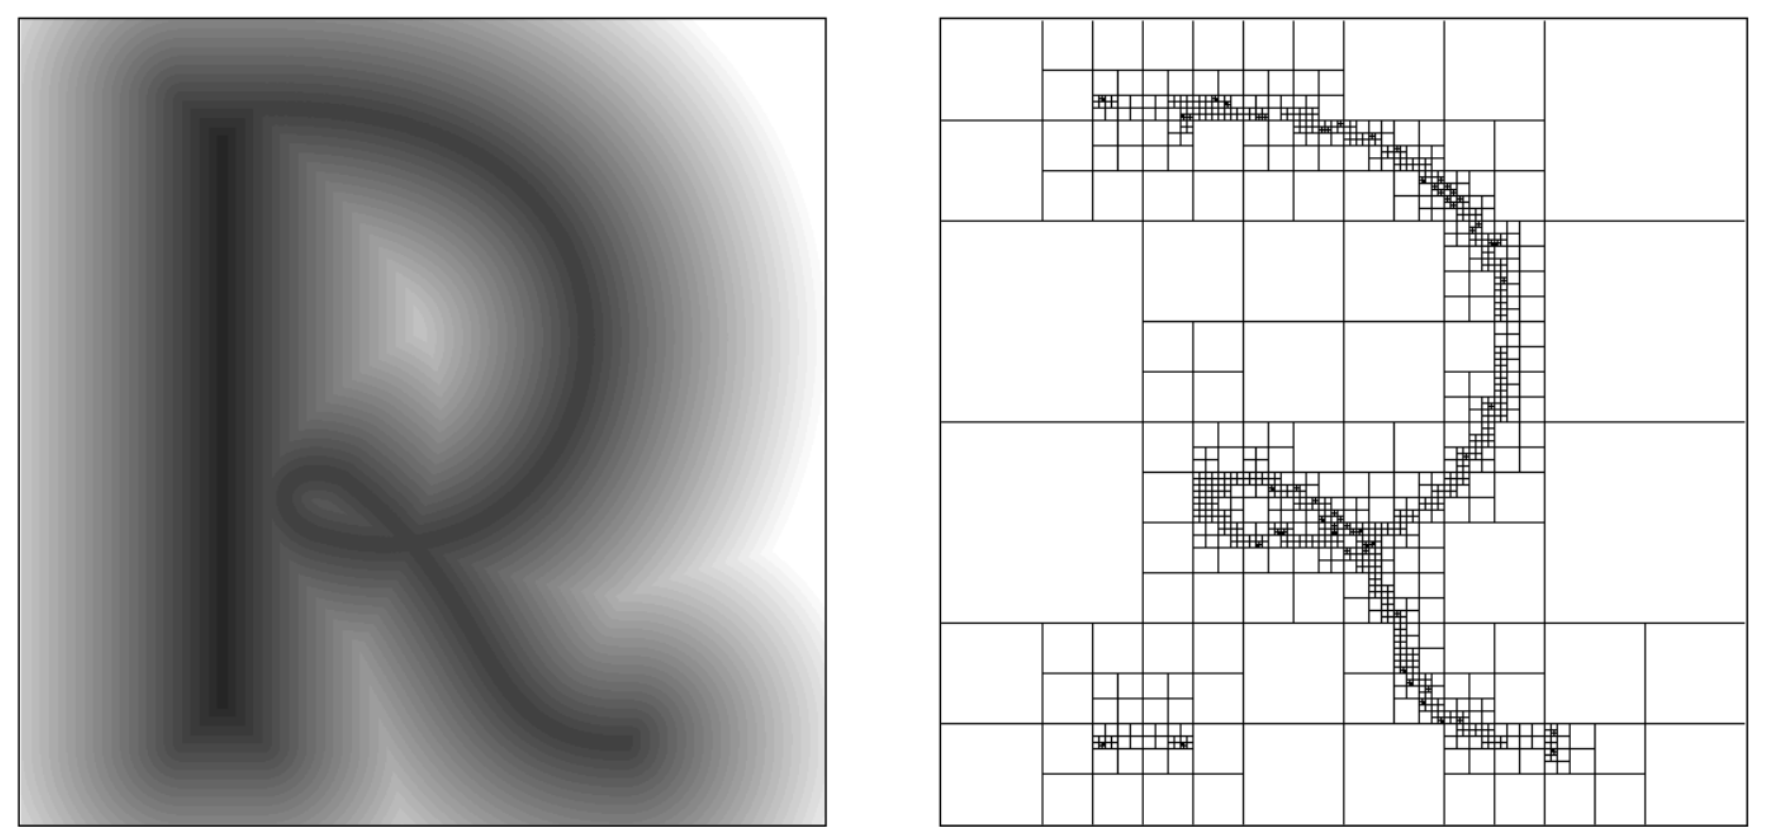
\includegraphics[width=0.95\textwidth]{figures/asdf.png}
    \caption{2d representation of ASDF}
    \label{fig:asdf}
  \end{figure}
  \scriptsize Borrowed from: \textit{Adaptively Sampled Distance Fields: A General Representation of Shape for Computer Graphics}
\end{frame}
\begin{frame}
  \frametitle{Hash-based methods}
\end{frame}
\begin{frame}
  \frametitle{Gigavoxels}
\end{frame}
\subsection{Dictionary-based sampling of SDFs}
\begin{frame}
  \frametitle{Inspiration: Compression and Rendering of Point Clouds}
  \begin{figure}
    \centering
    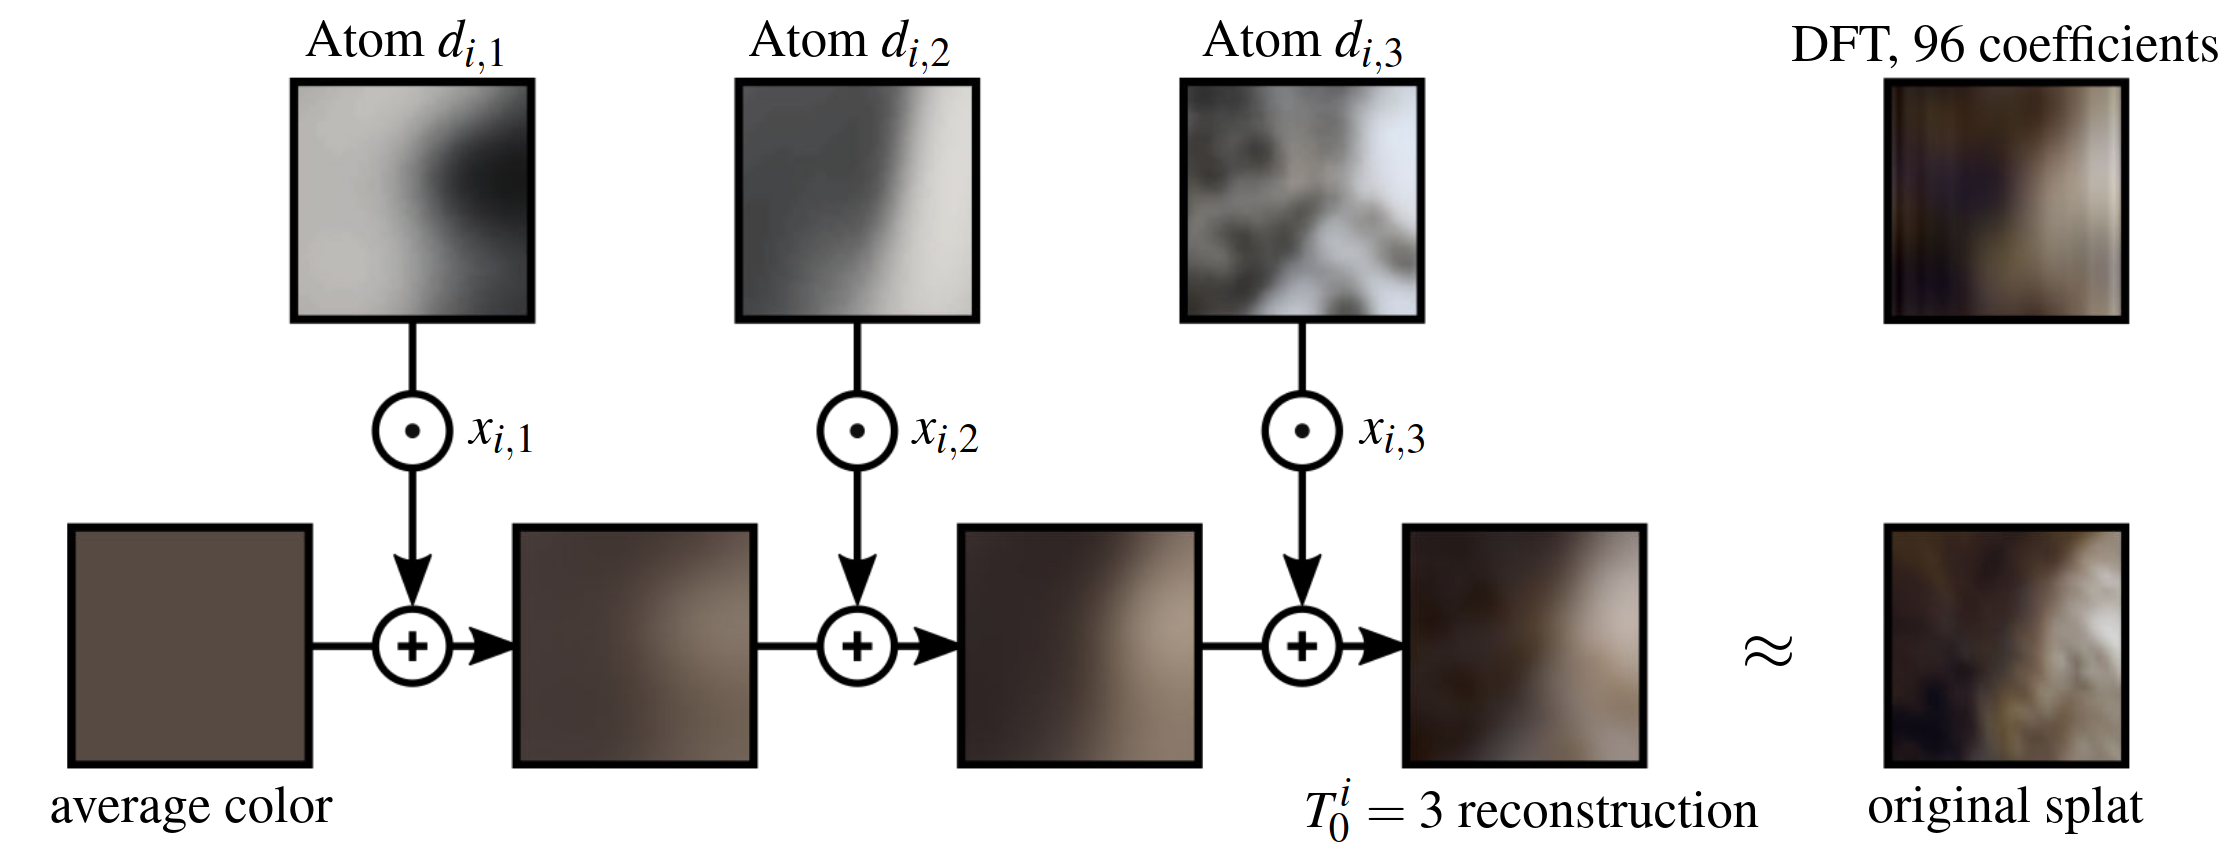
\includegraphics[width=0.95\textwidth]{figures/point-cloud-splat.png}
    \caption{Sparse coding of point cloud texture splats}
    \label{fig:spoint-cloud-splat}
  \end{figure}
  \scriptsize Borrowed from: \textit{Compression and Rendering of Textured Point Clouds via Sparse Coding}
\end{frame}
\begin{frame}
  \frametitle{Proposed representation}
  \begin{figure}
    \centering
    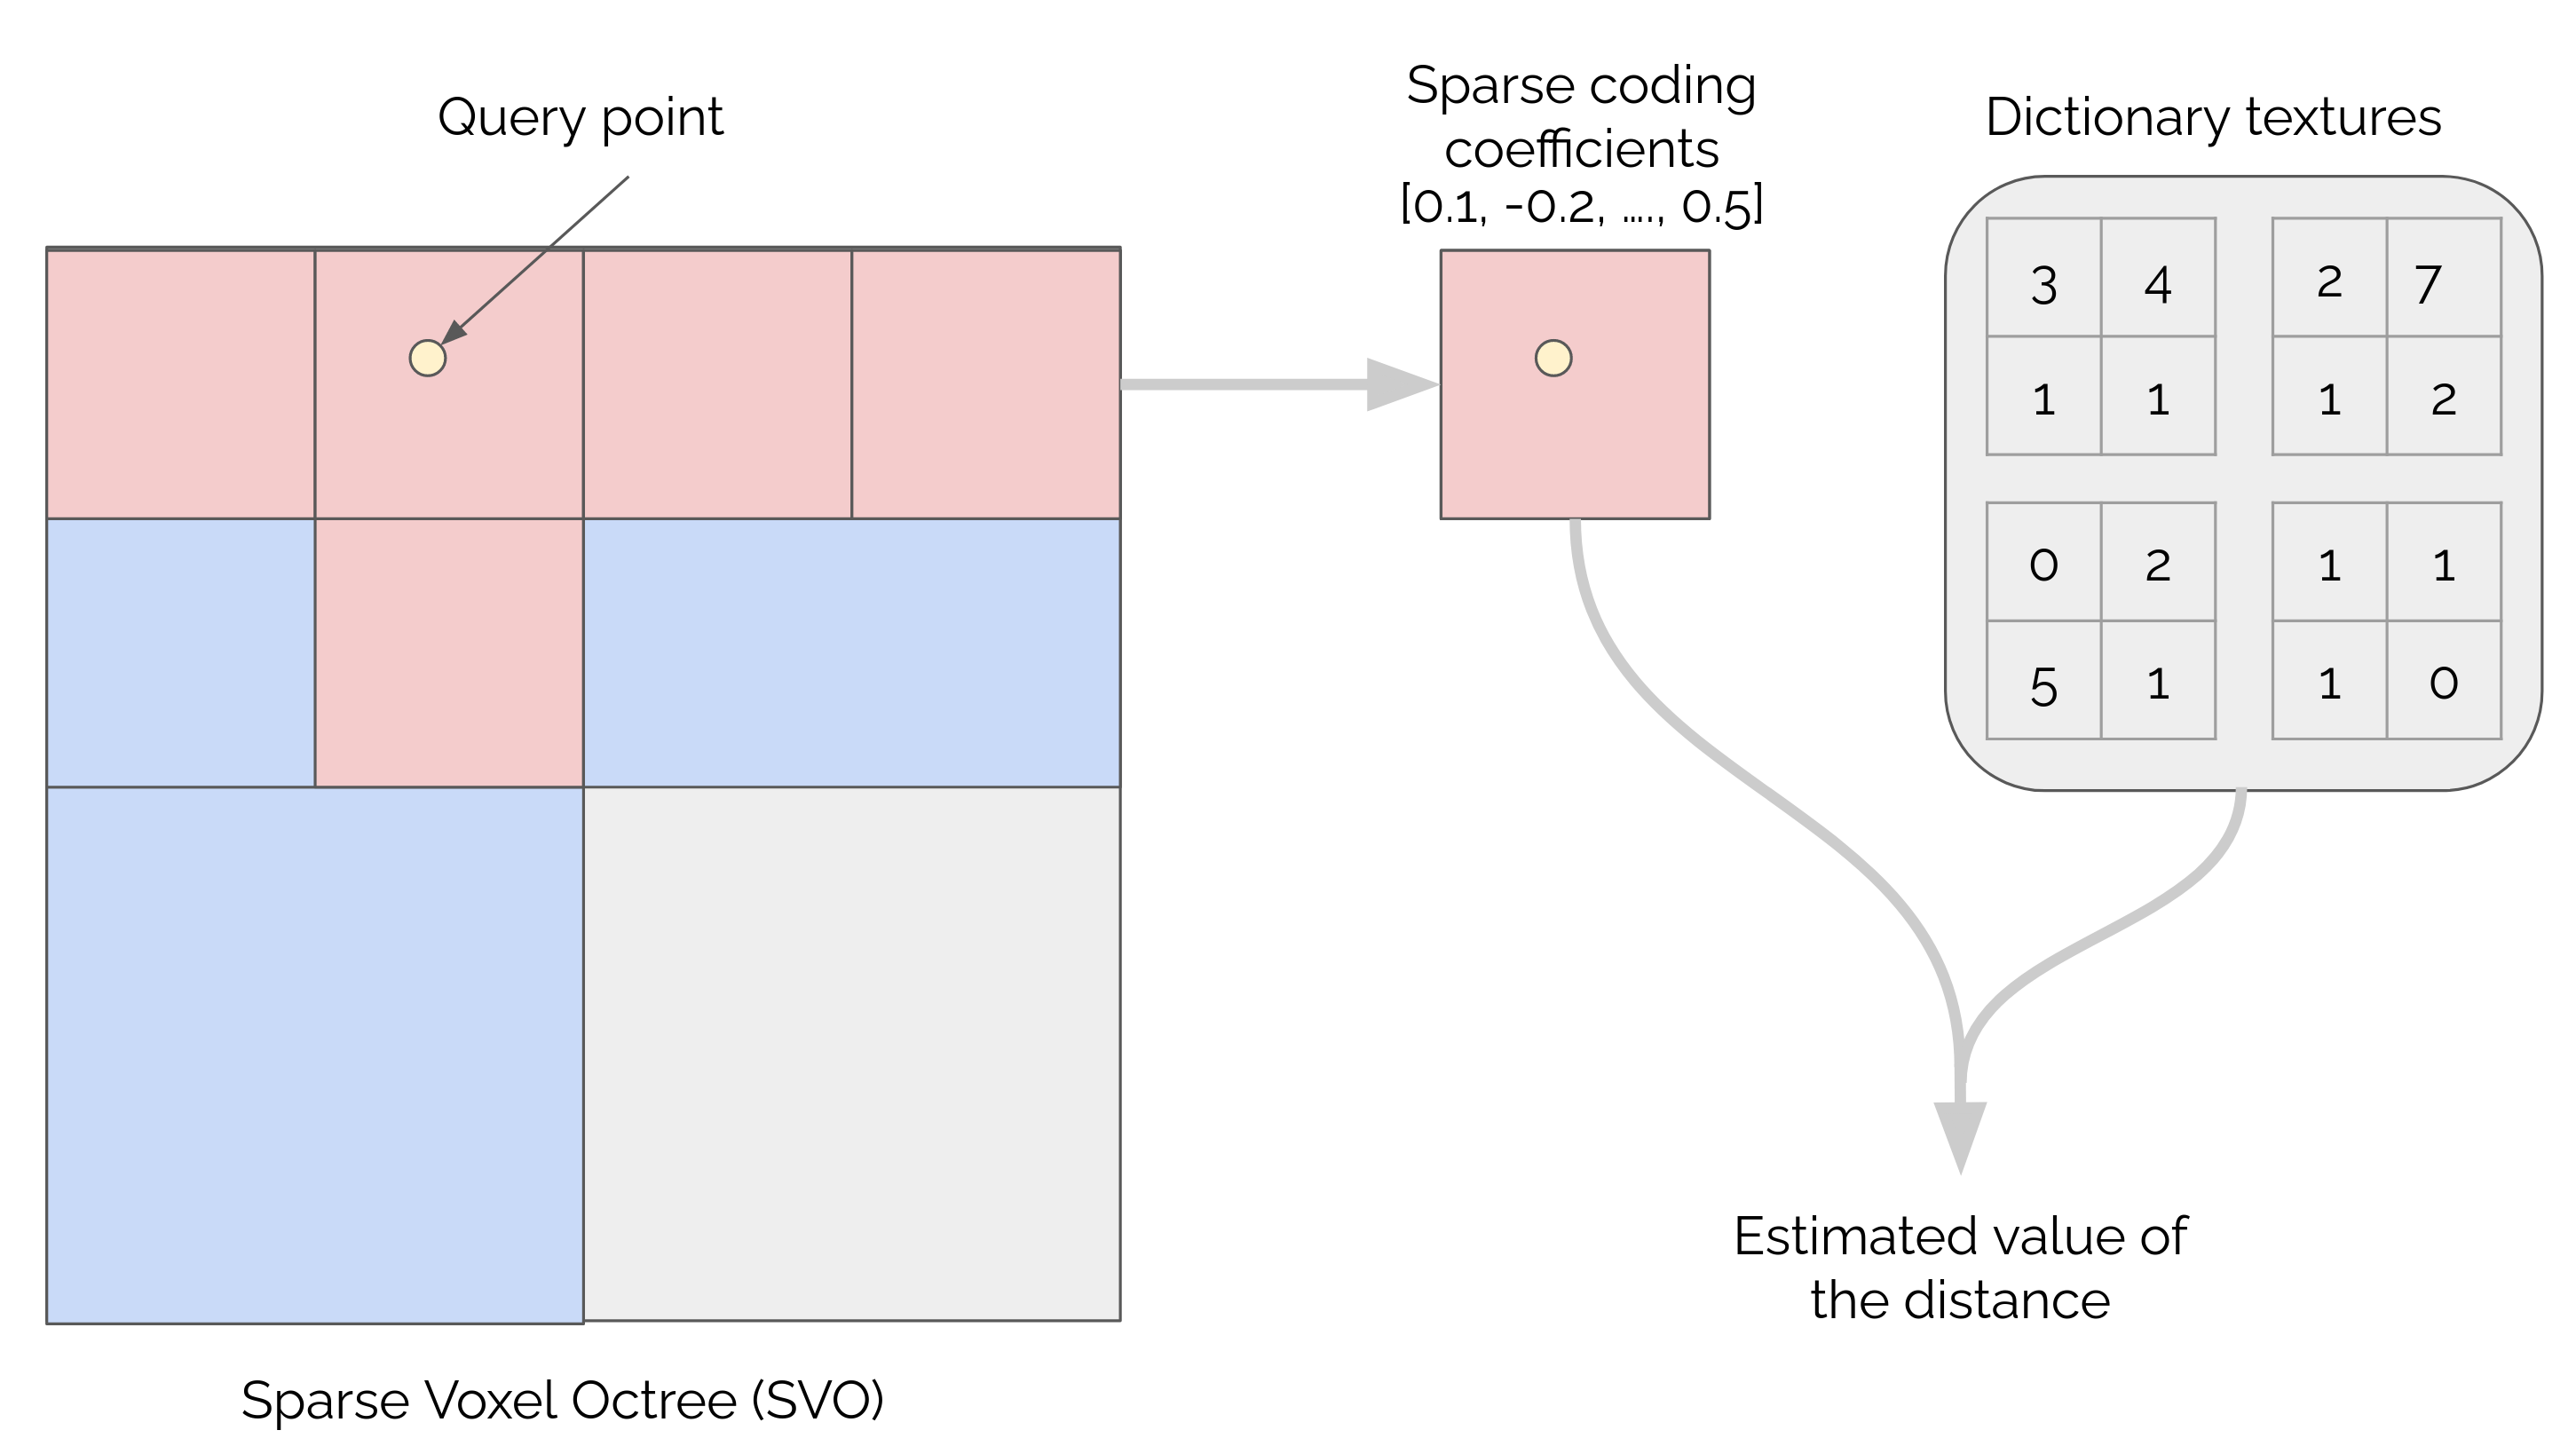
\includegraphics[width=0.95\textwidth]{figures/sparse-coding-sdf.png}
    \caption{Proposed dictionary-based representation of the SDF}
    \label{fig:sparse-coding-sdf}
  \end{figure}
\end{frame}

\subsection{Neural representations of SDFs}
\begin{frame}
  \frametitle{Representing SDF locally as learned features}
  \begin{figure}
    \centering
    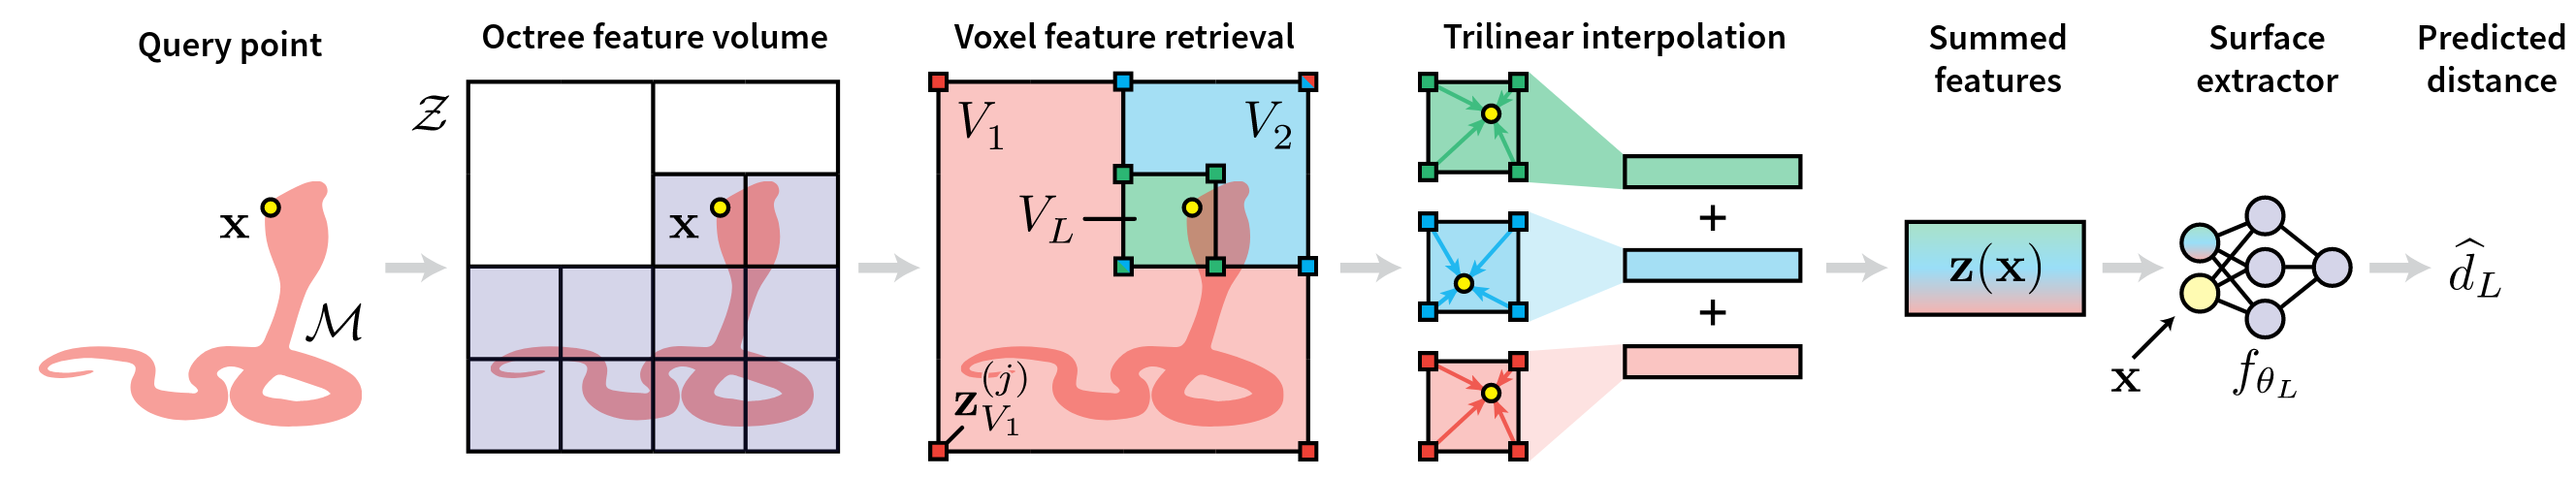
\includegraphics[width=0.95\textwidth]{figures/neural-sdf.png}
    \caption{Architecture proposed in \textit{Neural Geometric Level of Detail: Real-time Rendering with Implicit 3D Shapes}}
    \label{fig:neural-sdf}
  \end{figure}
\end{frame}


\section{Generating SDFs}

\end{document}